\chapter{Spectroscopies de rotation et de vibration}\label{ch:b3:rovibrational-spectroscopy}

Sur un haut plateau aride, des dizaines d'antennes radio pointent vers un
nuage sombre entre les étoiles. Parmi les fréquences qu'elles recueillent
figure une raie à
\qty{115.271}{GHz}~: des molécules de monoxyde de carbone, à quelques
kelvins, qui passent de leur premier niveau de rotation au plus bas. De
ce seul nombre, un chimiste tire la longueur de la liaison C--O à une
fraction de picomètre près~; de l'intensité des raies suivantes, la
température du nuage. Les rotations et les vibrations des molécules sont
l'objet de ce chapitre~: leurs niveaux, issus du rotateur et de
l'oscillateur du
\cref{ch:b3:quantum-model-systems}~; les règles de sélection, issues du
\cref{ch:b3:group-theory-applied}~; et ce que mesurent les spectres ---
longueurs de liaison, \omterm{def:b3:quantum-model-systems:oscillator}{constantes de force}, énergies de dissociation.

\begin{recall}
Le \Cref{ch:b3:quantum-model-systems} a donné le \omterm{def:b3:quantum-model-systems:rotor}{rotateur rigide},
$E_J = J(J+1)\hbar^2/2I$
de \omterm{def:b3:quantum-model-systems:degenerate}{dégénérescence} $2J + 1$, et l'\omterm{def:b3:quantum-model-systems:oscillator}{oscillateur harmonique}, $E_v = (v + \frac12)h\nu$,
pour une molécule diatomique de \omterm{def:b3:quantum-model-systems:oscillator}{masse réduite} $\mu$. Le
\Cref{ch:b3:group-theory-applied} a énoncé les règles de sélection
infrarouge et Raman. Le volume de première année a mesuré des spectres
infrarouges en nombres d'onde et défini la polarisabilité d'une molécule.
\end{recall}

\begin{omfigure}
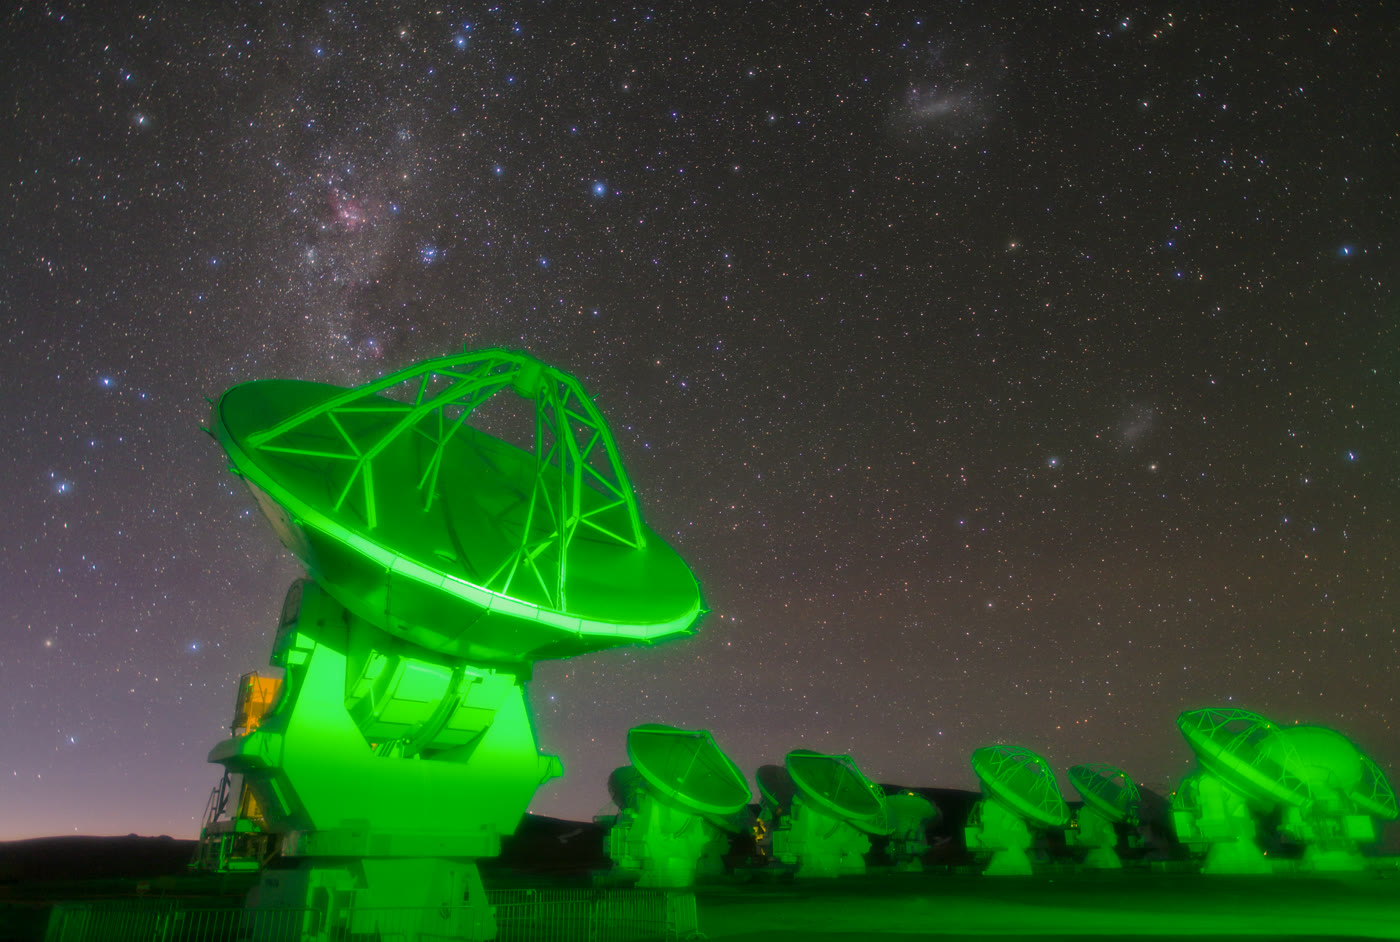
\includegraphics[width=0.7\linewidth]{images/book4/alma-antennas.jpg}

{\small Antennes d'un interféromètre radio sur un haut plateau~: elles
enregistrent, parmi bien d'autres, les raies de rotation du monoxyde de
carbone des nuages interstellaires. Photographie ESO/B.~Tafreshi
(twanight.org), CC BY 4.0.}
\end{omfigure}

\section{Spectres de rotation}

\begin{definition}[Constante de rotation, isotopologue]\label{def:b3:rovibrational-spectroscopy:rotational-constant}
La \emph{constante de rotation}\index{constante de rotation} d'une
molécule linéaire est $B = h/(8\pi^2cI)$, en \unit{cm^{-1}} (ou
$B = h/8\pi^2I$ en hertz), de sorte que ses niveaux de rotation sont
$F(J) = BJ(J+1)$ en nombres d'onde. Des molécules qui ne diffèrent que
par les isotopes de leurs atomes sont des \emph{isotopologues}\index{isotopologue}
(\ce{^{12}C^{16}O}, \ce{^{13}C^{16}O})~; dans l'\omterm{def:b3:computational-chemistry:born-oppenheimer}{approximation de
Born--Oppenheimer}, elles ont les mêmes longueurs de liaison et les mêmes
\omterm{def:b3:quantum-model-systems:oscillator}{constantes de force}.
\end{definition}

\begin{definition}[Règles de sélection générale et spécifique]\label{def:b3:rovibrational-spectroscopy:selection}
Une \emph{règle de sélection générale}\index{regle de selection generale@règle de sélection générale} énonce la
propriété qu'une molécule doit posséder pour présenter un type de spectre~;
une \emph{règle de sélection spécifique}\index{regle de selection specifique@règle de sélection spécifique}
énonce les variations de nombre quantique permises.
\end{definition}

\begin{proposition}[Spectres de rotation pure]\label{prop:b3:rovibrational-spectroscopy:rotational-lines}
Une molécule n'a de spectre de rotation pure (micro-ondes) que si elle
possède un moment dipolaire permanent~; pour une molécule linéaire, la
règle spécifique est $\Delta J
= \pm1$. Les raies d'absorption se situent à
\[
\tilde\nu = F(J+1) - F(J) = 2B(J + 1), \qquad J = 0, 1, 2, \dots,
\]
également espacées de $2B$.
\end{proposition}

\begin{proof}
L'interaction avec la lumière passe par le moment dipolaire~: une
molécule sans dipôle permanent n'a pas de dipôle oscillant quand elle
tourne. La règle $\Delta J
= \pm1$ provient de l'annulation de $\int Y_{J'M'}^*\cos\theta\,Y_{JM}$
sauf si $J' = J
\pm 1$ (la composante du dipôle selon $z$ se transforme comme
$Y_{1,0}$), admise.
Alors $B(J+1)(J+2) - BJ(J+1) = 2B(J+1)$.
\end{proof}

\begin{method}[Longueur de liaison à partir d'une raie de rotation]\label{met:b3:rovibrational-spectroscopy:bond-length}
\begin{enumerate}
  \item De la raie $J + 1 \leftarrow J$ de fréquence $\nu$, déduire $B =
        \nu/2(J+1)$ (en hertz).
  \item Calculer le moment d'inertie $I = h/8\pi^2B$.
  \item Avec la \omterm{def:b3:quantum-model-systems:oscillator}{masse réduite} tirée des masses isotopiques, $r = \sqrt{I/\mu}$.
\end{enumerate}
\end{method}

\begin{example}[Le monoxyde de carbone]\label{ex:b3:rovibrational-spectroscopy:co}
% ledger: rotl:CO.1-0, imass:O16
La raie $J = 1 \leftarrow 0$ de \ce{^{12}C^{16}O} est à \qty{115271.20}{MHz}~:
$B = \qty{57635.6}{MHz} = \qty{1.92252}{cm^{-1}}$, $I = \qty{1.4560e-46}{kg.m^2}$.
Avec $\mu = 12 \times 15.99491/27.99491 = \qty{6.85621}{u}$, $r_0 = \qty{113.09}{pm}$.
Ce $r_0$ est une moyenne de la liaison sur sa vibration de point zéro, un
peu plus longue que la longueur d'équilibre $r_e$
(\cref{sec:b3:rovibrational-spectroscopy:real-bonds}).
\end{example}

\begin{definition}[Constante de distorsion centrifuge]\label{def:b3:rovibrational-spectroscopy:centrifugal}
Une liaison en rotation s'allonge~; les niveaux deviennent
$F(J) = BJ(J+1) - DJ^2(J+1)^2$,
où $D$ est la \emph{constante de distorsion centrifuge}\index{constante de distorsion centrifuge},
et les raies $2B(J+1) - 4D(J+1)^3$ se resserrent lentement aux
grands $J$.
\end{definition}

\begin{proposition}[La raie la plus intense]\label{prop:b3:rovibrational-spectroscopy:jmax}
Si les intensités des raies suivent la population du niveau inférieur, $(2J+1)
\eu^{-hcBJ(J+1)/kT}$, le niveau le plus peuplé se situe vers
\[
J_{\max} \approx \sqrt{\frac{kT}{2hcB}} - \frac12.
\]
\end{proposition}

\begin{proof}
Traitons $J$ comme une variable continue et dérivons~: $\frac{\dd}{\dd J}[(2J+1)\eu^{-aJ(J+1)}]
= [2 - a(2J+1)^2]\eu^{-aJ(J+1)}$ avec $a = hcB/kT$~; la dérivée s'annule
pour $(2J + 1)^2 =
2/a$.
\end{proof}

\begin{omfigure}
\begin{tikzpicture}
\begin{axis}[width=0.9\linewidth, height=4.8cm, xmin=0, xmax=70, ymin=0,
  ymax=1.12, ytick=\empty, axis x line=bottom, axis y line=left, ycomb,
  xlabel={nombre d'onde / cm$^{-1}$}, ylabel={intensité relative},
  tick label style={font=\small}, label style={font=\small}]
\addplot[omDef, very thick] table[x=nu, y=I] {figdata/out/bachelor-3-rotational-spectrum-co-30.dat};
\addplot[omThm, thick, xshift=1.2pt] table[x=nu, y=I] {figdata/out/bachelor-3-rotational-spectrum-co-300.dat};
\end{axis}
\end{tikzpicture}

{\small Le spectre d'absorption de rotation du monoxyde de carbone, raies
espacées de $2B = \qty{3.845}{cm^{-1}}$, intensités prises égales à la
population du niveau inférieur, à \qty{30}{K} (bleu) et à \qty{300}{K}
(rouge, légèrement décalé pour la lisibilité), chaque température étant
rapportée à sa raie la plus intense. À \qty{30}{K}, la raie la plus
intense est
$J = 3 \leftarrow 2$~; à \qty{300}{K}, $J = 8 \leftarrow 7$.}
\end{omfigure}

\section{Vibrations des liaisons réelles}\label{sec:b3:rovibrational-spectroscopy:real-bonds}

Une liaison réelle n'obéit pas à la loi de Hooke loin de l'équilibre~:
elle s'assouplit quand on l'étire, puis se rompt.

\begin{definition}[Potentiel de Morse]\label{def:b3:rovibrational-spectroscopy:morse}
Le \emph{potentiel de Morse}\index{potentiel de Morse} est $V(r) = D_e[1 -
\eu^{-\beta(r - r_e)}]^2$~: harmonique près de $r_e$ (\omterm{def:b3:quantum-model-systems:oscillator}{constante de force}
$2\beta^2D_e$), il tend vers la limite de dissociation $D_e$ aux grands
$r$.
\end{definition}

\begin{proposition}[Niveaux de l'oscillateur de Morse]\label{prop:b3:rovibrational-spectroscopy:morse-levels}
En nombres d'onde, les niveaux de vibration d'un oscillateur de Morse sont
\[
G(v) = \tilde\omega_e(v + \tfrac12) - \tilde\omega_ex_e(v + \tfrac12)^2, \qquad
\tilde\omega_ex_e = \frac{\tilde\omega_e^2}{4D_e},
\]
une échelle dont les barreaux se resserrent et s'arrêtent à $v_{\max} = \lfloor\tilde\omega_e/
2\tilde\omega_ex_e - \frac12\rfloor$.
\end{proposition}
\admitted

La résolution de l'équation de Morse relève de cours plus avancés~; les
niveaux sont vérifiés numériquement dans les données de figure de ce
chapitre.

\begin{definition}[Constante d'anharmonicité, transition fondamentale, bande harmonique, bande chaude]\label{def:b3:rovibrational-spectroscopy:anharmonic}
$\tilde\omega_ex_e$ est la \emph{constante d'anharmonicité}\index{constante d'anharmonicite@constante d'anharmonicité}.
La \emph{transition fondamentale}\index{transition fondamentale}
est $v = 1 \leftarrow 0$~; une \emph{bande harmonique}\index{bande harmonique} correspond à $v = n \leftarrow 0$
avec $n \ge 2$, faible parce que la règle $\Delta v = \pm1$ de
l'\omterm{def:b3:quantum-model-systems:oscillator}{oscillateur harmonique} n'est que légèrement violée~; une \emph{bande
chaude}\index{bande chaude} part d'un niveau excité, $v = 2 \leftarrow 1$,
et croît avec la température.
\end{definition}

\begin{definition}[Énergie de dissociation spectroscopique]\label{def:b3:rovibrational-spectroscopy:dissociation}
L'\emph{énergie de dissociation spectroscopique}\index{energie de dissociation spectroscopique@énergie de dissociation spectroscopique}
d'une molécule est la profondeur de son potentiel, $D_e$, mesurée depuis
le minimum, ou $D_0 = D_e - G(0)$, mesurée depuis le niveau le plus bas
--- par molécule et à \qty{0}{K}, contrairement à l'enthalpie de
dissociation de liaison du volume de deuxième année, qui est une
enthalpie molaire à \qty{298}{K}.
\end{definition}

\begin{corollary}[$D_e$ et $D_0$ d'un oscillateur de Morse]\label{cor:b3:rovibrational-spectroscopy:de}
$D_e = \tilde\omega_e^2/4\tilde\omega_ex_e$ et $D_0 = D_e - (\frac12\tilde\omega_e -
\frac14\tilde\omega_ex_e)$.
\end{corollary}

\begin{proof}
La première est la relation de la proposition~; la seconde est $G(0)$.
\end{proof}

\begin{proposition}[Extrapolation de Birge--Sponer]\label{prop:b3:rovibrational-spectroscopy:birge-sponer}
Les écarts $\Delta G(v + \frac12) = G(v+1) - G(v) = \tilde\omega_e - 2\tilde\omega_ex_e(v +
1)$ décroissent linéairement avec $v$~; leur somme jusqu'à ce qu'ils
s'annulent donne $D_0$, l'aire sous la courbe de $\Delta G$ en fonction
de $v$.
\end{proposition}

\begin{proof}
Retrancher les deux expressions de $G$. $D_0$ est l'énergie qui sépare
$v = 0$ de la limite, la somme de tous les écarts.
\end{proof}

\begin{example}[Le chlorure d'hydrogène]\label{ex:b3:rovibrational-spectroscopy:hcl}
% ledger: diat:HCl.we, diat:HCl.wexe, janaf:H.dfH0, janaf:Cl.dfH0, janaf:HCl.dfH0
Pour \ce{H^{35}Cl}, $\tilde\omega_e = \qty{2990.95}{cm^{-1}}$ et $\tilde\omega_ex_e =
\qty{52.82}{cm^{-1}}$~: la \omterm{def:b3:rovibrational-spectroscopy:anharmonic}{transition fondamentale} est à $\tilde\omega_e - 2\tilde\omega_ex_e =
\qty{2885.3}{cm^{-1}}$ et la première \omterm{def:b3:rovibrational-spectroscopy:anharmonic}{bande harmonique} à $2\tilde\omega_e - 6\tilde\omega_ex_e =
\qty{5665.0}{cm^{-1}}$, un peu moins que le double de la fondamentale. Le
modèle de Morse prévoit $D_e = \qty{42342}{cm^{-1}}$ et
$D_0 = \qty{40860}{cm^{-1}}$~; le vrai $D_0$,
tiré des enthalpies de formation de H, Cl et HCl à \qty{0}{K}, vaut
\qty{35760}{cm^{-1}} (\qty{4.43}{eV}). Le potentiel réel s'aplatit plus
vite qu'une courbe de Morse ajustée sur le fond~: les extrapolations de
Birge--Sponer à partir des niveaux les plus bas surestiment les énergies
de dissociation.
\end{example}

\begin{omfigure}
\begin{tikzpicture}
\begin{axis}[name=morse, width=0.55\linewidth, height=6cm, xmin=0.8, xmax=4.0,
  ymin=0, ymax=48000, axis lines=left, xlabel={$r$ / \AA}, ylabel={$V$ / cm$^{-1}$},
  unbounded coords=jump, scaled y ticks=false, ytick={0,10000,20000,30000,40000},
  tick label style={font=\small}, label style={font=\small}]
\addplot[black, thick] table[x=r, y=V] {figdata/out/bachelor-3-morse-levels.dat};
\addplot[gray, dashed] table[x=r, y=harm] {figdata/out/bachelor-3-morse-levels.dat};
\addplot[omDef] table[x=r, y=E] {figdata/out/bachelor-3-morse-levels-levels.dat};
\draw[<->, omThm] (axis cs:3.7,0) -- (axis cs:3.7,42342) node[pos=0.5, left, font=\small] {$D_e$};
\draw[dashed, omThm] (axis cs:1.2,42342) -- (axis cs:4.0,42342);
\end{axis}
\begin{axis}[at={(morse.east)}, anchor=west, xshift=1.6cm, width=0.4\linewidth,
  height=5cm, xmin=0, xmax=28, ymin=0, ymax=3100, axis lines=left,
  xlabel={$v$}, ylabel={$\Delta G(v + \frac12)$ / cm$^{-1}$},
  tick label style={font=\small}, label style={font=\small}]
\addplot[omDef, only marks, mark size=1.2pt] table[x=v, y=dG] {figdata/out/bachelor-3-morse-levels-bs.dat};
\addplot[omDef!40, fill=omDef!12, draw=none] table[x=v, y=dG] {figdata/out/bachelor-3-morse-levels-bs.dat} \closedcycle;
\end{axis}
\end{tikzpicture}

{\small À gauche~: le \omterm{def:b3:rovibrational-spectroscopy:morse}{potentiel de Morse} de \ce{HCl} construit à partir
de ses constantes spectroscopiques (trait plein), la parabole harmonique
de même courbure (en tirets), et un niveau de vibration sur trois, tracé
entre ses points de rebroussement~; les niveaux se resserrent vers $D_e$.
À droite~: le diagramme de Birge--Sponer des écarts~; l'aire grisée vaut
$D_0$.}
\end{omfigure}

\section{Bandes de rotation-vibration}

Une transition de vibration d'un gaz s'accompagne de changements de
rotation, $\Delta
J = \pm1$ pour une molécule diatomique dans un état ${}^1\Sigma$.

\begin{definition}[Branches P, Q et R, origine de la bande]\label{def:b3:rovibrational-spectroscopy:branches}
Dans une bande de rotation-vibration, les raies telles que
$\Delta J = -1$ forment la \emph{branche
P}\index{branche P}, celles telles que $\Delta J = +1$ la \emph{branche R}\index{branche R},
et celles telles que $\Delta J = 0$, quand elles sont permises, la
\emph{branche Q}\index{branche Q}.
L'\emph{origine de la bande}\index{origine de la bande} $\tilde\nu_0$ est
la différence d'énergie de vibration sans rotation.
\end{definition}

\begin{theorem}[Différences de combinaison]\label{thm:b3:rovibrational-spectroscopy:combination-differences}
Avec les \omterm{def:b3:rovibrational-spectroscopy:rotational-constant}{constantes de rotation} $B_0$ et $B_1$ des niveaux de vibration
inférieur et supérieur, $R(J) = \tilde\nu_0 + B_1(J+1)(J+2) - B_0J(J+1)$ et $P(J) = \tilde\nu_0 +
B_1(J-1)J - B_0J(J+1)$, et
\[
R(J - 1) - P(J + 1) = 4B_0(J + \tfrac12), \qquad R(J) - P(J) = 4B_1(J + \tfrac12).
\]
\end{theorem}

\begin{proof}
Les deux premières découlent de $E = G(v) + B_vJ(J+1)$ pour les deux
niveaux. $R(J - 1)$ et
$P(J + 1)$ aboutissent au même niveau supérieur $J$, depuis les niveaux
inférieurs $J - 1$ et $J + 1$~:
leur différence vaut $B_0[(J+1)(J+2) - (J-1)J] = B_0(4J + 2)$. De même,
$R(J)$ et
$P(J)$ partent du même niveau inférieur et aboutissent à $J + 1$ et
$J - 1$.
\end{proof}

\begin{method}[Analyser une bande de rotation-vibration]\label{met:b3:rovibrational-spectroscopy:combination}
\begin{enumerate}
  \item Repérer la lacune~: pour une molécule diatomique ${}^1\Sigma$, il
        n'y a pas de \omterm{def:b3:rovibrational-spectroscopy:branches}{branche Q}, et
        $\tilde\nu_0$ se trouve dans la lacune, entre $R(0)$ et $P(1)$.
  \item Numéroter les raies à partir de la lacune, vers l'extérieur~:
        $R(0), R(1), \dots$ et $P(1),
        P(2), \dots$.
  \item Utiliser les différences de combinaison pour obtenir $B_0$ et
        $B_1$
        séparément, puis $\alpha_e = B_0 - B_1$ et $B_e = B_0 + \frac12\alpha_e$.
\end{enumerate}
\end{method}

\begin{omfigure}
\begin{tikzpicture}
\begin{axis}[width=0.92\linewidth, height=5cm, xmin=2650, xmax=3080, ymin=0,
  ymax=1.15, ytick=\empty, axis x line=bottom, axis y line=left,
  xlabel={nombre d'onde / cm$^{-1}$}, ylabel={absorbance (relative)},
  tick label style={font=\small}, label style={font=\small}]
\addplot[omDef, thin] table[x=nu, y=A] {figdata/out/bachelor-3-rovib-band.dat};
\node[font=\small] at (axis cs:2780,1.06) {branche P};
\node[font=\small] at (axis cs:2985,1.06) {branche R};
\draw[->, gray] (axis cs:2885.3,0.45) -- (axis cs:2885.3,0.05);
\node[font=\small, gray, anchor=south] at (axis cs:2885.3,0.45) {$\tilde\nu_0$};
\end{axis}
\end{tikzpicture}

{\small La bande fondamentale de \ce{HCl} gazeux à \qty{300}{K},
calculée à partir de ses constantes spectroscopiques~: \omterm{def:b3:rovibrational-spectroscopy:branches}{branches P} et R
de part et d'autre de la lacune située à l'\omterm{def:b3:rovibrational-spectroscopy:branches}{origine de la bande}. Chaque
raie est un doublet, \ce{H^{35}Cl} et le \ce{H^{37}Cl}, plus faible et
un peu plus bas (abondances naturelles 76\,\% et 24\,\%). Les raies R se
resserrent,
les raies P s'écartent, parce que $B_1 < B_0$.}
\end{omfigure}

\begin{example}[Les constantes de \ce{HCl} tirées de sa bande]\label{ex:b3:rovibrational-spectroscopy:analysis}
% ledger: diat:HCl.Be, diat:HCl.ae
Avec $R(0) = \qty{2905.58}{cm^{-1}}$ et $P(2) = \qty{2842.94}{cm^{-1}}$, on trouve
$6B_0 = \qty{62.64}{cm^{-1}}$, donc $B_0 = \qty{10.440}{cm^{-1}}$. Avec $R(1) = 2925.23$ et $P(1) =
\qty{2864.43}{cm^{-1}}$, $B_1 = \qty{10.133}{cm^{-1}}$. Donc $\alpha_e = \qty{0.307}{cm^{-1}}$
et $B_e = \qty{10.593}{cm^{-1}}$, les valeurs à partir desquelles la
bande a été construite~: la méthode les retrouve exactement.
\end{example}

\section{La spectroscopie Raman}

\begin{definition}[Diffusions Raman et Rayleigh]\label{def:b3:rovibrational-spectroscopy:raman}
Quand une lumière de fréquence $\nu_0$ traverse un échantillon, la plus
grande partie de la lumière diffusée garde la fréquence $\nu_0$~: c'est
la \emph{diffusion Rayleigh}\index{diffusion Rayleigh}.
Une petite fraction est décalée des fréquences de rotation ou de
vibration des molécules~: c'est la \emph{diffusion Raman}\index{diffusion Raman}.
Les raies de plus basse fréquence sont les \emph{raies Stokes}\index{raie Stokes} (la
molécule a gagné de l'énergie), celles de plus haute fréquence les
\emph{raies anti-Stokes}\index{raie anti-Stokes} (elle en a perdu).
\end{definition}

\begin{proposition}[Origine classique de l'effet Raman]\label{prop:b3:rovibrational-spectroscopy:raman-classical}
Si la polarisabilité d'une molécule qui vibre à $\nu_{\mathrm{vib}}$ varie
selon $\alpha = \alpha_0 + \alpha_1\cos(2\pi\nu_{\mathrm{vib}}t)$, le
dipôle induit par un
champ $E_0\cos(2\pi\nu_0t)$ oscille à $\nu_0$ et à $\nu_0 \pm \nu_{\mathrm{vib}}$.
Une vibration n'est \omterm{def:b3:group-theory-applied:activity}{active en Raman} que si elle fait varier la
polarisabilité.
\end{proposition}

\begin{proof}
$\mu = \alpha E = \alpha_0E_0\cos(2\pi\nu_0t) + \frac12\alpha_1E_0[\cos2\pi(\nu_0 +
\nu_{\mathrm{vib}})t + \cos2\pi(\nu_0 - \nu_{\mathrm{vib}})t]$, d'après $\cos a\cos b =
\frac12[\cos(a+b) + \cos(a-b)]$. Chaque dipôle oscillant rayonne à sa
propre fréquence~; sans $\alpha_1$, seul subsiste le terme Rayleigh.
\end{proof}

\begin{proposition}[Raies Raman de rotation]\label{prop:b3:rovibrational-spectroscopy:rotational-raman}
Une molécule linéaire de polarisabilité anisotrope présente des raies
Raman de rotation telles que $\Delta J = \pm2$, décalées de la raie
excitatrice de
\[
|\Delta\tilde\nu| = F(J+2) - F(J) = 4B(J + \tfrac32) = 6B, 10B, 14B, \dots
\]
--- la première raie à $6B$, puis un espacement de $4B$.
\end{proposition}

\begin{proof}
L'ellipsoïde de polarisabilité d'une molécule linéaire en rotation
reprend la même orientation deux fois par tour, donc il module la
diffusion au double de la fréquence de rotation~: $\Delta J = \pm2$ (la
règle quantique, admise). Alors
$B(J+2)(J+3) - BJ(J+1) = B(4J + 6)$.
\end{proof}

\begin{example}[Le diazote vu par Raman]\label{ex:b3:rovibrational-spectroscopy:n2}
% ledger: diat:N2.Be, diat:N2.ae
\ce{N2} n'a pas de dipôle et pas de spectre infrarouge ni micro-ondes,
mais sa polarisabilité est anisotrope~: ses raies Raman de rotation
commencent à $6B_0 =
\qty{11.94}{cm^{-1}}$ de la raie excitatrice et sont espacées de
\qty{7.96}{cm^{-1}}. Leurs intensités alternent dans le rapport 2:1
entre $J$ pairs et impairs~: les deux noyaux \ce{^{14}N} sont
identiques, et la statistique de spin nucléaire
(\cref{ch:b3:statistical-thermo-applied}) donne aux niveaux de $J$ pair
un poids double de celui des niveaux impairs.
\end{example}

\begin{omfigure}
\begin{tikzpicture}
\begin{axis}[name=r, width=0.55\linewidth, height=4.6cm, xmin=-110, xmax=110,
  ymin=0, ymax=1.1, ytick=\empty, axis x line=bottom, axis y line=left, ycomb,
  xlabel={déplacement Raman / cm$^{-1}$}, tick label style={font=\small}, label style={font=\small},
  title={\small \ce{N2}, Raman de rotation, \qty{300}{K}}]
\addplot[omDef, thick] table[x=shift, y=I] {figdata/out/bachelor-3-rotational-spectrum-n2-raman.dat};
\draw[gray, thick] (axis cs:0,0) -- (axis cs:0,1.05);
\end{axis}
\begin{scope}[xshift=0.6\linewidth, font=\small]
  \draw[omstate] (0,0) -- (2.4,0) node[right] {$v = 0$};
  \draw[omstate] (0,1.0) -- (2.4,1.0) node[right] {$v = 1$};
  \draw[omvib, densely dashed] (0,3.2) -- (2.4,3.2) node[right] {virtuel};
  \draw[omabs] (0.3,0) -- (0.3,3.18);
  \draw[omfluo] (0.5,3.18) -- (0.5,0.02);
  \node[font=\scriptsize, omThm, anchor=east] at (0.22,1.6) {Rayleigh};
  \draw[omabs] (1.3,0) -- (1.3,3.18);
  \draw[omphos] (1.5,3.18) -- (1.5,1.02) node[pos=0.4, right, font=\scriptsize] {Stokes};
\end{scope}
\end{tikzpicture}

{\small À gauche~: le spectre Raman de rotation du diazote calculé à
\qty{300}{K}~: \omterm{def:b3:rovibrational-spectroscopy:raman}{raies Stokes} aux déplacements positifs (à droite), \omterm{def:b3:rovibrational-spectroscopy:raman}{raies
anti-Stokes} aux déplacements négatifs (à gauche, un peu plus faibles),
avec l'alternance 2:1 des intensités~; le trait gris en zéro marque la
raie Rayleigh, bien plus intense. À droite~: schéma énergétique des
\omterm{def:b3:rovibrational-spectroscopy:raman}{diffusions Rayleigh} et Stokes
par un niveau virtuel (qui n'est pas un état réel de la molécule).}
\end{omfigure}

\section{Molécules polyatomiques}

\begin{definition}[Types de rotateurs]\label{def:b3:rovibrational-spectroscopy:rotor-types}
Une molécule dont les trois moments principaux d'inertie sont égaux est
une \emph{toupie sphérique}\index{toupie spherique@toupie sphérique} (\ce{CH4}, \ce{SF6})~; avec deux
moments égaux, une
\emph{toupie symétrique}\index{toupie symetrique@toupie symétrique} (\ce{NH3}, \ce{CHCl3}, \ce{C6H6})~;
avec trois moments différents, une \emph{toupie asymétrique}\index{toupie asymetrique@toupie asymétrique}
(\ce{H2O}, la plupart des molécules)~; les molécules linéaires ont un
moment nul.
\end{definition}

Une \omterm{def:b3:rovibrational-spectroscopy:rotor-types}{toupie sphérique} n'a ni dipôle ni spectre de rotation~; une \omterm{def:b3:rovibrational-spectroscopy:rotor-types}{toupie
symétrique} a pour niveaux $BJ(J+1) + (A - B)K^2$, où $K$ compte le moment
cinétique autour de son axe,
et des raies qui tombent encore à $2B(J+1)$ puisque $\Delta K = 0$~; une
\omterm{def:b3:rovibrational-spectroscopy:rotor-types}{toupie asymétrique}
a un spectre irrégulier, ajusté par ordinateur. Les vibrations des
molécules polyatomiques sont leurs modes normaux, nommés et sélectionnés
au
\cref{ch:b3:group-theory-applied}~: le spectre infrarouge montre les
modes qui se transforment comme $x$, $y$, $z$, chacun avec sa propre
structure de rotation.

\begin{inthelab}[Une cellule à gaz dans un spectromètre infrarouge]
Le \ce{HCl} gazeux est admis dans une cellule de \qty{10}{cm} munie de
fenêtres transparentes à l'infrarouge, à l'intérieur d'un spectromètre à
transformée de Fourier. À une résolution de \qty{1}{cm^{-1}},
les \omterm{def:b3:rovibrational-spectroscopy:branches}{branches P} et R apparaissent comme des raies simples~; à
\qty{0.25}{cm^{-1}}, chacune se dédouble en son doublet
\ce{H^{35}Cl}/\ce{H^{37}Cl}, distant de \qty{2}{cm^{-1}}. Le chlorure
d'hydrogène est toxique et corrosif~: la cellule est remplie sur une
rampe à vide, sous hotte.
\end{inthelab}

\begin{safety}{\ghs[0.8cm]{GHS04}\ghs[0.8cm]{GHS05}\ghs[0.8cm]{GHS06}}
Chlorure d'hydrogène gazeux~: gaz sous pression, corrosif pour la peau,
les yeux et les voies respiratoires, toxique par inhalation. Manipulé
uniquement en appareillage clos ou sous hotte.
\end{safety}

\begin{history}[Raman, 1928]
En 1928, C. V. Raman et K. S. Krishnan observèrent, dans la lumière du
Soleil filtrée par un filtre violet et diffusée par des liquides, une
faible lumière d'une autre couleur qu'un filtre vert croisé permettait
d'isoler. Raman reçut le prix Nobel de physique 1930~; les sources laser
firent de son effet une technique d'analyse courante cinquante ans plus
tard.
\end{history}

\section{Exercices}

\begin{exercise}[$\star$]\label{exo:b3:rovibrational-spectroscopy:1}
% ledger: imass:O16
À partir de $B_0 = \qty{1.9225}{cm^{-1}}$ pour \ce{^{12}C^{16}O}, calculer
le moment d'inertie et la longueur de liaison $r_0$.
\end{exercise}

\begin{exercise}[$\star$]\label{exo:b3:rovibrational-spectroscopy:2}
% ledger: diat:HCl.Be, diat:HCl.ae
Avec $B_0 = \qty{10.440}{cm^{-1}}$, donner les positions des quatre
premières raies du spectre de rotation de \ce{H^{35}Cl} et le $J$ de la
raie la plus intense à
\qty{300}{K}.
\end{exercise}

\begin{exercise}[$\star$]\label{exo:b3:rovibrational-spectroscopy:3}
Parmi \ce{H2}, \ce{HCl}, \ce{N2}, \ce{CO2}, \ce{CH4}, \ce{SF6} et
\ce{H2O}, lesquelles présentent un spectre d'absorption de rotation
pure~? Un spectre Raman de rotation~?
\end{exercise}

\begin{exercise}[$\star$]\label{exo:b3:rovibrational-spectroscopy:4}
% ledger: diat:HCl.we, diat:HCl.wexe
Quelle fraction des molécules de \ce{HCl} se trouve dans $v = 1$ à 300 et
à \qty{1000}{K} (\omterm{def:b3:rovibrational-spectroscopy:anharmonic}{transition fondamentale} à \qty{2885.3}{cm^{-1}})~? Quand la
\omterm{def:b3:rovibrational-spectroscopy:anharmonic}{bande chaude} devient-elle visible~?
\end{exercise}

\begin{exercise}[$\star\star$]\label{exo:b3:rovibrational-spectroscopy:5}
La \omterm{def:b3:rovibrational-spectroscopy:anharmonic}{transition fondamentale} et la première \omterm{def:b3:rovibrational-spectroscopy:anharmonic}{bande harmonique} de
\ce{H^{35}Cl} se situent à 2885.3 et
\qty{5665.0}{cm^{-1}}. En déduire $\tilde\omega_e$ et $\tilde\omega_ex_e$.
\end{exercise}

\begin{exercise}[$\star\star$]\label{exo:b3:rovibrational-spectroscopy:6}
Avec les constantes de l'exercice précédent, calculer $D_e$ et $D_0$ du
modèle de Morse, et les comparer au vrai $D_0 = \qty{35760}{cm^{-1}}$.
Convertir les deux valeurs de
$D_0$ en \unit{kJ/mol}.
\end{exercise}

\begin{exercise}[$\star\star$]\label{exo:b3:rovibrational-spectroscopy:7}
Quatre raies de la bande fondamentale de \ce{H^{35}Cl} sont
$R(0) = 2905.58$, $R(1) = 2925.23$,
$P(1) = 2864.43$ et $P(2) = \qty{2842.94}{cm^{-1}}$. Trouver $B_0$, $B_1$,
$\alpha_e$ et
l'\omterm{def:b3:rovibrational-spectroscopy:branches}{origine de la bande}.
\end{exercise}

\begin{exercise}[$\star\star$]\label{exo:b3:rovibrational-spectroscopy:8}
% ledger: imass:H1, imass:H2, imass:Cl35
Prévoir $B_0$ et l'\omterm{def:b3:rovibrational-spectroscopy:branches}{origine de la bande} de \ce{D^{35}Cl} à partir de ceux
de \ce{H^{35}Cl}, à l'aide des
\omterm{def:b3:quantum-model-systems:oscillator}{masses réduites} ($\tilde\omega_e \propto \mu^{-1/2}$, $\tilde\omega_ex_e \propto
\mu^{-1}$, $B \propto \mu^{-1}$).
\end{exercise}

\begin{exercise}[$\star\star$]\label{exo:b3:rovibrational-spectroscopy:9}
% ledger: diat:N2.Be, diat:N2.ae
Pour \ce{N2}, $B_0 = \qty{1.9896}{cm^{-1}}$. Donner les déplacements des
trois premières raies Raman Stokes de rotation, et expliquer
l'alternance de leurs intensités.
\end{exercise}

\begin{exercise}[$\star\star\star$]\label{exo:b3:rovibrational-spectroscopy:10}
% ledger: rotl:CO.1-0, rotl:CO.2-1, rotl:CO.3-2
Les trois premières raies de rotation de \ce{^{12}C^{16}O} sont à
115271.2018,
230538.0000 et \qty{345795.9899}{MHz}. Montrer qu'un \omterm{def:b3:quantum-model-systems:rotor}{rotateur rigide} ne
rend pas compte de ces valeurs, et déterminer $B$ et la \omterm{def:b3:rovibrational-spectroscopy:centrifugal}{constante de
distorsion centrifuge} $D$.
\end{exercise}

\begin{exercise}[$\star\star\star$]\label{exo:b3:rovibrational-spectroscopy:11}
Montrer que la somme de Birge--Sponer des écarts $\Delta G(v + \frac12)$
d'un oscillateur de Morse, de $v = 0$ au dernier niveau lié, est proche
de $D_e - G(0)$, et évaluer cette somme pour \ce{HCl}.
\end{exercise}

\begin{exercise}[$\star\star\star$]\label{exo:b3:rovibrational-spectroscopy:12}
Le noyau \ce{^{16}O} a un spin nul, si bien que les niveaux de
\ce{^{16}O^{12}C^{16}O} de
$J$ impair n'existent pas. Quel est l'espacement de ses raies Raman de
rotation, et le déplacement de la première, en fonction de $B$~?
Pourquoi \ce{CO2} n'a-t-il pas de spectre micro-ondes~?
\end{exercise}

\section{Problème~: à l'écoute d'un nuage froid}

\begin{problem}[{Problème du week-end --- la longueur de liaison du
monoxyde de carbone tirée de sa première raie de rotation, la
température d'un nuage interstellaire, l'isotopologue carbone 13, et la
bande infrarouge}]
\label{pb:b3:rovibrational-spectroscopy:1}
% ledger: rotl:CO.1-0, rotl:CO.2-1, rotl:13CO.1-0, imass:O16, imass:C13, iso:C13, diat:CO.we, diat:CO.wexe, re:CO
Données~: raies de \ce{^{12}C^{16}O} $J = 1 \leftarrow 0$ à \qty{115.2712}{GHz} et $2
\leftarrow 1$ à \qty{230.5380}{GHz}~; raie $1 \leftarrow 0$ de
\ce{^{13}C^{16}O} à
\qty{110.2014}{GHz}~; masses \ce{^{12}C} 12 (exactement), \ce{^{13}C} 13.00335,
\ce{^{16}O} \qty{15.99491}{u}~; abondance naturelle de \ce{^{13}C}
1.1\,\%~; pour \ce{^{12}C^{16}O},
$\tilde\omega_e = \qty{2169.81}{cm^{-1}}$, $\tilde\omega_ex_e = \qty{13.288}{cm^{-1}}$, et
la longueur d'équilibre $r_e = \qty{112.83}{pm}$. $h = \qty{6.62607e-34}{J.s}$, $u =
\qty{1.66054e-27}{kg}$, $c = \qty{2.99792e10}{cm/s}$, $hc/k = \qty{1.43878}{cm.K}$.

\medskip\noindent\textbf{Partie I --- La liaison.}
\begin{enumerate}
  \item Calculer $B_0$ en hertz et en \unit{cm^{-1}}.
  \item Calculer la \omterm{def:b3:quantum-model-systems:oscillator}{masse réduite} de \ce{^{12}C^{16}O} en kilogrammes.
  \item Calculer le moment d'inertie.
  \item En déduire $r_0$.
  \item Comparer à $r_e$. Pourquoi $r_0$ est-il plus long~?
  \item Prévoir la raie $2 \leftarrow 1$ pour un \omterm{def:b3:quantum-model-systems:rotor}{rotateur rigide}.
        Commenter la valeur mesurée.
\end{enumerate}

\medskip\noindent\textbf{Partie II --- La température du nuage.}
\begin{enumerate}[resume]
  \item Donner les énergies, en \unit{cm^{-1}} et en kelvins ($E/k$), des
        niveaux $J =
        0$, 1, 2.
  \item Écrire le rapport des populations $N_2/N_1$ à la température $T$.
  \item Les observations donnent $N_2/N_1 = 0.85$ (données du problème).
        Trouver $T$.
  \item Quel niveau est le plus peuplé à cette température~?
  \item Pourquoi un tel nuage ne peut-il pas être observé dans la bande
        infrarouge de vibration~?
  \item Pourquoi la raie $1 \leftarrow 0$ est-elle le traceur le plus
        utilisé du gaz froid~?
\end{enumerate}

\medskip\noindent\textbf{Partie III --- L'\omterm{def:b3:rovibrational-spectroscopy:rotational-constant}{isotopologue}.}
\begin{enumerate}[resume]
  \item Calculer la \omterm{def:b3:quantum-model-systems:oscillator}{masse réduite} de \ce{^{13}C^{16}O}.
  \item Prévoir sa raie $1 \leftarrow 0$ à partir de celle de \ce{^{12}C^{16}O}.
  \item Comparer à la valeur mesurée, \qty{110.2014}{GHz}. Qu'a-t-on
        négligé~?
  \item Si les deux raies étaient faibles et non saturées, quel rapport
        de leurs intensités les abondances naturelles donneraient-elles~?
  \item Le rapport observé est bien plus petit. Qu'en déduire sur la raie
        de \ce{^{12}C^{16}O}~?
  \item Pourquoi observe-t-on en pratique les deux \omterm{def:b3:rovibrational-spectroscopy:rotational-constant}{isotopologues}
        ensemble~?
\end{enumerate}

\medskip\noindent\textbf{Partie IV --- La bande de vibration.}
\begin{enumerate}[resume]
  \item Calculer l'\omterm{def:b3:rovibrational-spectroscopy:branches}{origine de la bande} fondamentale, en \unit{cm^{-1}} et
        en micromètres.
  \item Calculer la première \omterm{def:b3:rovibrational-spectroscopy:anharmonic}{bande harmonique}.
  \item Calculer l'\omterm{def:b3:quantum-model-systems:oscillator}{énergie de point zéro}.
  \item Qu'est-ce qui sépare les premières raies R et P~?
  \item Laquelle des deux molécules, \ce{^{12}C^{16}O} ou \ce{^{13}C^{16}O},
        a l'origine de bande la plus basse~?
  \item Énoncer le résultat~: la longueur de liaison $r_0$ du monoxyde de
        carbone obtenue à partir d'une seule raie radio.
\end{enumerate}
\end{problem}
